\documentclass[preview]{standalone}

\usepackage{amsmath}
\usepackage{amssymb}
\usepackage{bettelini}
\usepackage{stellar}
\usepackage[version=4]{mhchem}

\hypersetup{
    colorlinks=true,
    linkcolor=black,
    urlcolor=blue,
    pdftitle={Chimica},
    pdfpagemode=FullScreen,
}

\begin{document}

\title{Chimica}
\id{chimica-termodinamica-chimica}
\genpage

\begin{snippetdefinition}{energia-attivazione-definizione}{Energia di attivazione}
    L'\textit{energia di attivazione} è l'energia necessaria
    a far accadere una reazione chimica.
\end{snippetdefinition}

\begin{snippetdefinition}{catalizzatore-definizione}{Catalizzatore}
    Un \textit{catalizzatore} è
    una sostanza in grado di influenzare la
    velocità di una reazione chimica senza essere consumata.
\end{snippetdefinition}

\begin{snippet}{catalizzatore-expl}
    Il catalizzatore accelera la reazione abbassando l'energia
di attivazione dando la possibilità che si realizzi un nuovo
percorso che porta ai prodotti, caratterizzato da uno stadio
cineticamente determinante con una minor energia di
attivazione rispetto a quello della reazione non catalizzata.
\end{snippet}

\begin{snippetdefinition}{velocita-reazione-definizione}{Velocità di reazione}
    Per rappresentare la \textit{velocità di reazione}, descriviamo la
    variazione nel tempo della concentrazione di una specie
    presente nell'equazione chimica
    \[
        v
        = - \frac{1}{a} \frac{d[A]}{dt}
        = - \frac{1}{b} \frac{d[B]}{dt}
        = \frac{1}{p} \frac{d[P]}{dt}
        = \frac{1}{q} \frac{d[Q]}{dt}
    \]
    dove \(a,b,p,q\) sono i coefficienti stechiometrici
    per i reagenti \(A\) e \(B\) e i prodotti \(P\) e \(Q\).
\end{snippetdefinition}

\section{Teoria degli urti efficaci}

\begin{snippetdefinition}{teoria-urti-definizione}{Teoria degli urti}
    La \textit{teoria degli urti}
    indica che 
    la velocità di una reazione è
    proporzionale al numero di urti efficaci che avvengono
    nell'unità di tempo fra le molecole dei reagenti.
    Un urto è \textit{efficace} solo se porta alla formazione delle
    molecole dei prodotti.
\end{snippetdefinition}

\begin{snippet}{toeria-urti-illustration}
    \begin{center}
    \begin{figure}[th]
        \centering
        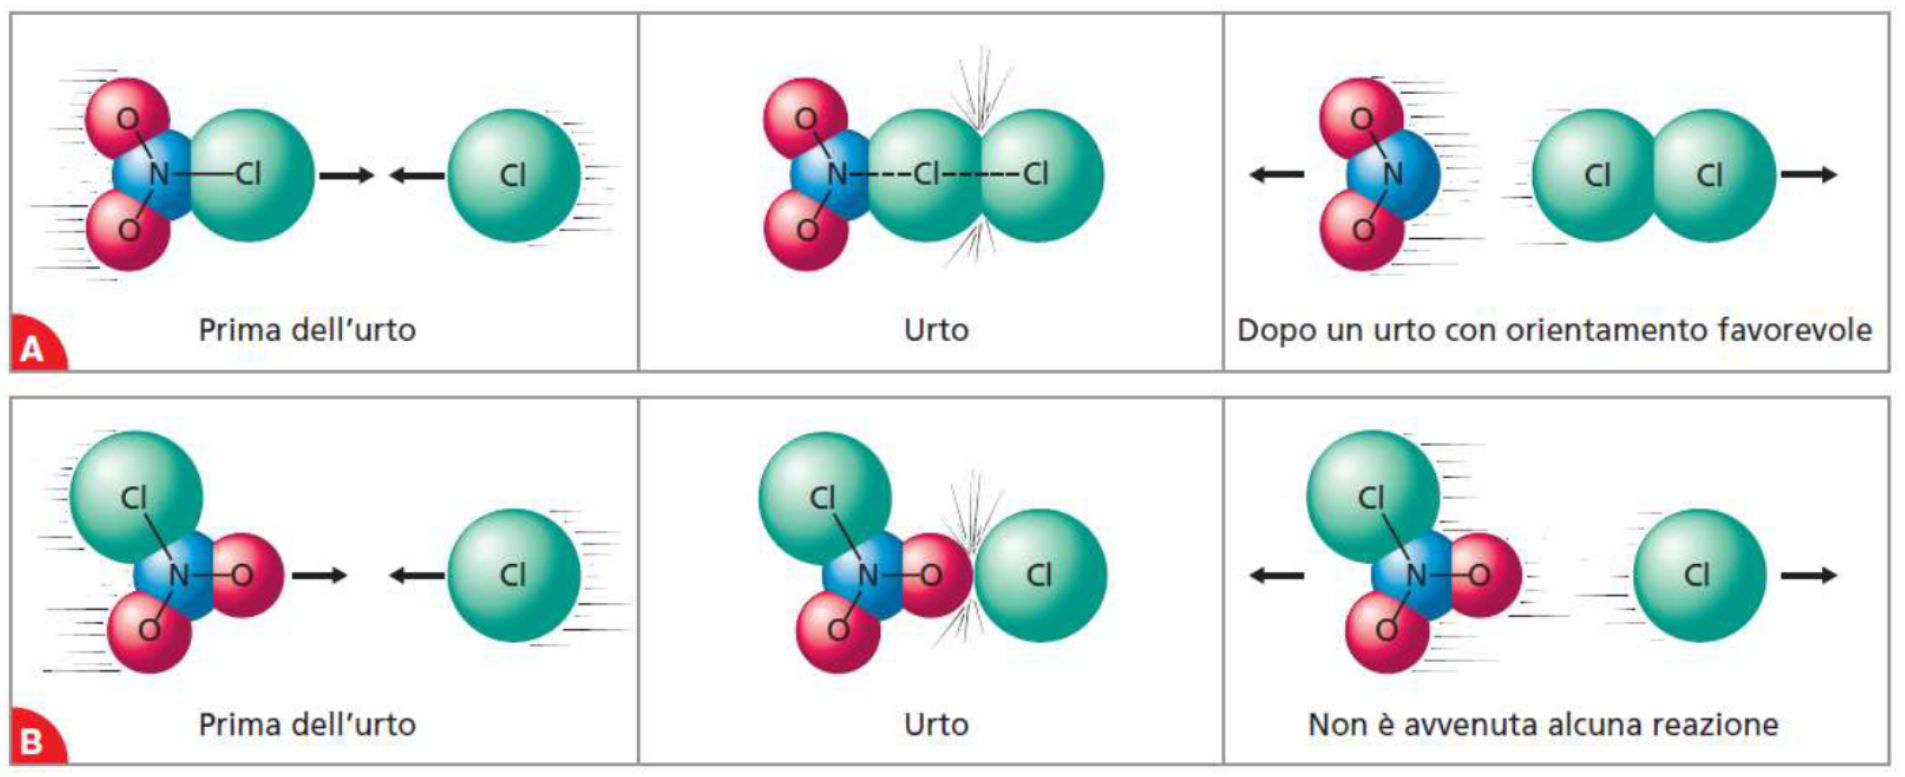
\includegraphics[width=\textwidth]{./resources/teoria-urti.png}
    \end{figure}
    \end{center}
\end{snippet}

\begin{snippet}{teoria-urti-expl1}
    Affinché gli urti siano efficaci occorre che le particelle che
entrano in contatto abbiano un'energia cinetica molecolare
minima, ossia l'energia di attivazione.

Dopo un urto, le molecole rallentano: la loro energia
cinetica diminuisce e si trasforma in energia potenziale.
\end{snippet}

\begin{snippetdefinition}{stato-transizione}{Stato di transizione}
    Con \textit{stato di transizione} si intende
    il momento della reazione in cui il
    legame tra i reagenti è parzialmente rotto e il nuovo
    legame è parzialmente formato (complesso attivato).
\end{snippetdefinition}

\plain{La sua energia corrisponde al punto più alto del diagramma dell'energia potenziale.}

\begin{snippet}{chem-reaction-illustration}
    \begin{center}
    \begin{figure}[th]
        \centering
        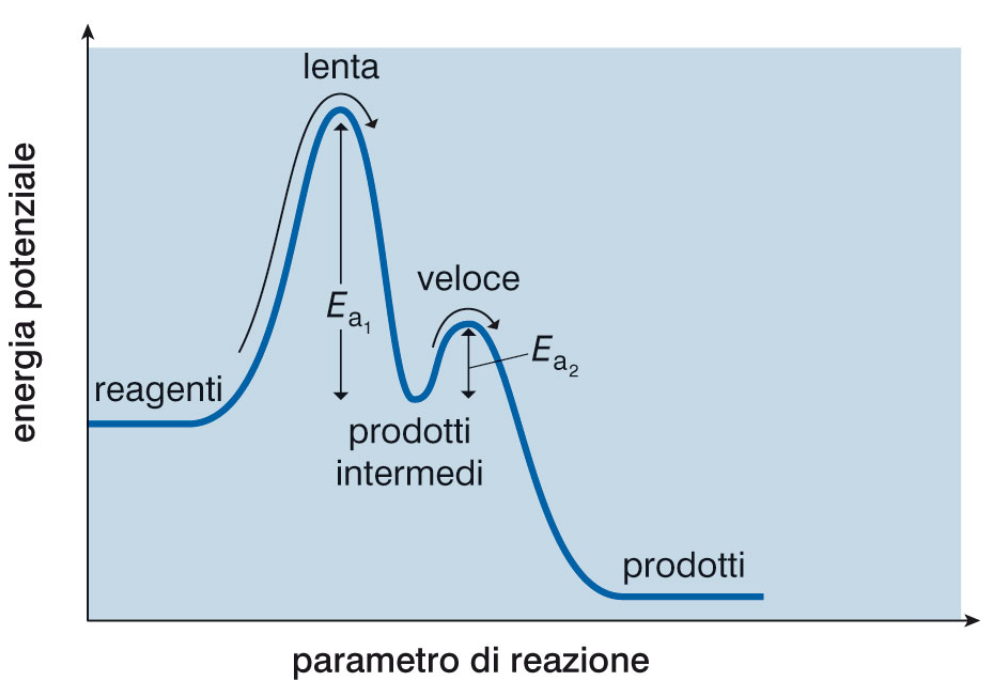
\includegraphics[width=\textwidth]{./resources/chem-reaction.png}
    \end{figure}
    \end{center}
\end{snippet}

\section{Equilibrio}

\begin{snippet}{equilibrio-expl1}
    In una reazione chimica, vi sono sia reazioni dirette che inverse.
Questo siginfica che è si giungere ad un equilibrio dove
il numero di reagenti e quello di prodotti tendono ad essere in equilibrio,
con scambi continui fra i due.
\end{snippet}

\begin{snippet}{equilibrio-illustration}
    \begin{center}
    \begin{figure}[th]
        \centering
        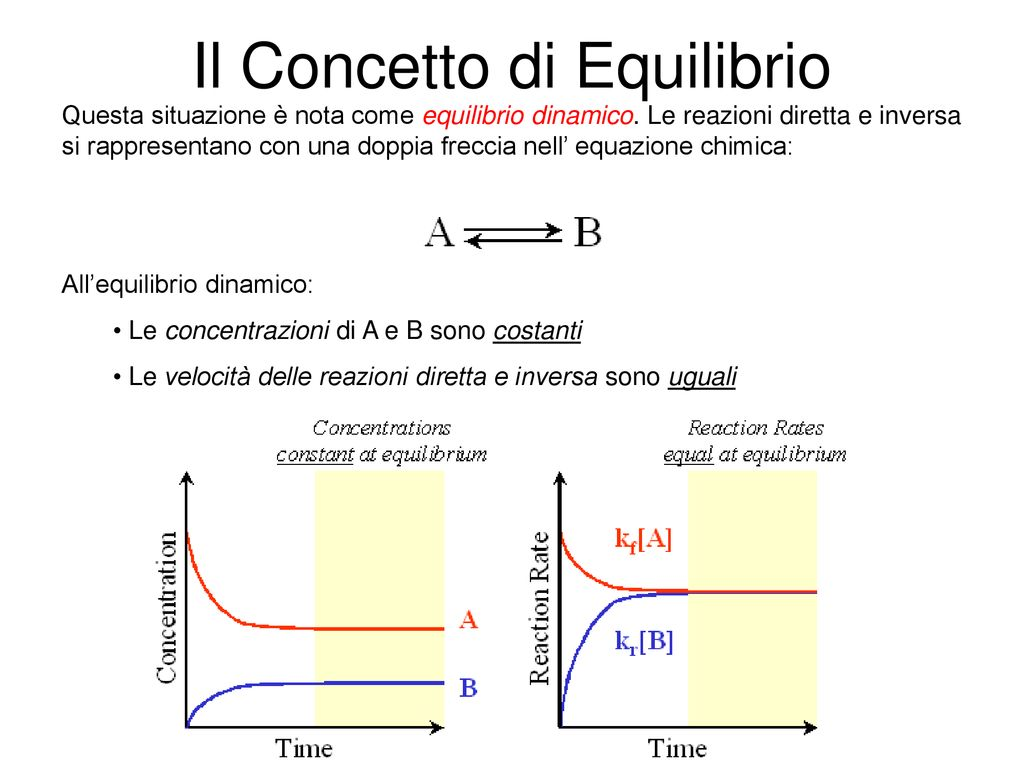
\includegraphics[width=\textwidth]{./resources/equilibrio}
    \end{figure}
    \end{center}
\end{snippet}

\begin{snippet}{equilibrio-expl2}
    Il grafico della reazione può essere quindi diviso in \textit{regione cinetica}
e \textit{regione di equilibrio}. 
Nell'equilibrio \textit{dinamico} le molecole continuano costantemente a
cambiare, e la velocità di reazione diretta diventa quella di reazione indiretta.
Nell'\textit{equilibrio statico} le reazioni si fermano.
\end{snippet}

% TODO: 2 reagenti e un prodotto. Possiamo cmq avere una regione di equilibrio
% Osserviamo che l'andamento di crescita e di diminuzione
% non è più speculare. Se ce ne sono solo 2 è speculare.

% Spostare una reazione verso destra, significa che il reagente si trasforma in prodotto.
% C'è più prodotto che reagente al momento dell'equilibrio.
% diagramma Alcuni diagrammi (RP) con le 3 immagini

\begin{snippetdefinition}{legge-di-azione-di-massa-definizione}{Legge di azione di massa}
    Data una reazione generica
    \[
        dD + eE \rightleftharpoons fF + gG
    \]
    l'\textit{espressione dell'azione di massa} è
    \[ \frac{{[F]}^g{[G]}^g}{{[D]}^d{[E]}^e} = K \]
    dove \(K\)  è la \textit{costante di equilibrio} e relaziona
    le concentrazioni delle singole specie chimiche all'equilibrio.
\end{snippetdefinition}

\begin{snippet}{costante-k-expl}
    Le dimensioni di \(K\) variano con la stechiometria della reazione.\\
Ogni reazione possiede una costante di equilibrio caratteristica,
il cui valore dipende solo dalla temperatura.

Se \(K\) è grande, la reazione è spostata a destra,
e vi sono pochi reagenti e tanti prodotti.
Di conseguenza, se il \(K\) è grandisimo la reazione inversa è quasi
ininfluente, perché ve n'è pochissima.
\end{snippet}

\begin{snippetexample}{creazione-ammoniaca}{Creazione ammoniaca}
    La creazione di ammoniaca \(NH_3\) possiede come reagenti \(N_2\) e \(H_2\).
    La reazione termochimica è data da
    \[
        N_{2(\text{g})} + H_{2(\text{g})}   \rightleftharpoons NH_{3(\text{g})}      
    \]
    Siccome abbiamo \(\Delta H = -46.2 \frac{\text{kJ}}{\text{mol}}\),
    possiamo convenientemente bilanciare l'equazione in maniera tale da avere 1 mole di ammoniaca
    \[
        \frac{1}{2}N_{2(\text{g})} + \frac{3}{2}H_{2(\text{g})}   \rightleftharpoons NH_{3(\text{g})}
    \]
    Partendo da un punto della reazione di equilibrio,
    aggiungere \(H_2\) o \(N_2\) porterà uno sbilanciamento dell'equilibrio.
    Di conseguenza,
    I valori di \(N_2\) e \(H_2\) diminuiranno, favorendo la creazione di ammoniaca.
    Allo stesso modo, togliere dell'ammoniaca porta alla creazione di nuova ammoniaca, a scapito
    di \(H_2\) e \(N_2\).
    Togliendo uno dei reagenti, la concentrazione di ammoniaca scende per riequilibrare la reazione,
    e quella dell'altro reagente sale, e viceversa.
    I rapporti fra le differenze di concentrazioni che bilanciano la reazione dopo
    uno squilibrio sono proporzionali ai coefficienti stechiometrici:
    togliendo dell'ammoniaca, la concentrazione di \(H_2\) diminuirà maggiormente di quella di \(N_2\).
\end{snippetexample}

\begin{snippet}{aumento-concentrazione-prodotto}
    I modi per aumentare la concentrazione di un prodotto sono:
\begin{enumerate}
    \item Aumentare i reagenti;
    \item Aumentare il volume del reattore;
    \item Aumentare la temperatura (se \(\Delta H > 0\)).
        Aumentando la temperatura,
        i prodotti aumentano se la reazione è endotermica (\(\Delta H > 0\)),
        mentre i prodotti diminuiscono se è esotermica (\(\Delta H < 0\));
    \item Aumentare la pressione (se ho più molti nei reagenti che nei prodotti).
        Se si aumenta la pressione, la miscela all'equilibrio
        cambia composizione e diminuisce il numero totale di molecole allo stato gassoso presenti nel recipiente.
        Non c'è effetto della pressione
        se non c'è variazione nel numero di molecole durante la reazione.
        L'aumento della pressione sposta l'equilirio verso la parte della reazione che possiede meno molti di gas.
        Questo è dato dal fatto che il sistema deve bilanciare l'aumento della pressione, spostando
        la reazione verso dove vi sono meno moli di gas (nei reagenti o nei prodotti);
    \item Togliere prodotto (per spostare l'equilibrio e fare generare altro prodotto, anche se meno di quanto ne ho tolto,
        ma il quantitativo totale aumenta).
\end{enumerate}

Il catalizzatore non aumenta la concentrazione di un prodotto, bensì solo la concentrazione.
La temperatura è l'unico fattore al quale cambia la costante \(K\).
\end{snippet}

\section{Principio di Le Chatelier}

\begin{snippetdefinition}{principio-le-chatelier}{Principio di Le Chatelier}
    Secondo \textit{principio di Le Chatelier},
    ogni sistema tende a reagire ad una perturbazione impostagli
    dall'esterno minimizzandone gli effetti.
\end{snippetdefinition}

\end{document}
